\documentclass[12pt, fleqn]{article}
\usepackage[serbian]{babel}


\usepackage{thesis}
\newcommand{\thesisName}{Hardverska implementacija Viola-Jones algoritma}

\author{Risto Pejašinović}
\date{}

\begin{document}
%% listing and figure numbering per section %%
\counterwithin{lstlisting}{section}
\counterwithin{figure}{section}
\counterwithin{equation}{section}
\counterwithin{table}{section}

\maketitle
\thispagestyle{empty}
\newpage

\tableofcontents
\newpage

\section{Viola-Jones algoritam}

\subsection{Uvod}

Namena algoritma je detekcija i lokalizacija objekata na slici. Osmišljen od
strane Paul Viola i Michael Jones 2001. godine \cite{Viola2001RapidOD}.

Dugo godina je zbog brze i pouzdane detekcije bio standardan način detekcije
lica na slici. I danas je prisutan u velikom broju mobilnih telefona i
digitalnih kamera, ali danas postaje polako zamenjen konvolucionim neuronskim
mrežama. \\

Pouzdanost i brzina su postignuti uvođenjem tri ključna doprinosa:
\begin{itemize}

\item \textbf{Integralna slika} omogućava brzo izračunavanje obeležja.
\item \textbf{AdaBoost} algoritam za učenje, odabiranjem obeležja povećava
  brzinu i pouzdanost detekcije.
\item \textbf{Kaskadni klasifikator} Realizovanjem algoritma u kaskadama
  omogućava brzo odbacivanje pozadine slike kako je mala verovatnoća da će se tu
  naći lice. \\
\end{itemize}


\subsection{Integralna slika}

Kao jedan od ključnih delova algoritma, integralna slika omogućava izračunavanje
površine svakog pravougana obeležja u konstantnom vremenu.

Intenzitet piksela u integralnoj slici na poziciji x,y je zbir svih piksela koji
se nalaze gore i levo od pozicije x,y.

\begin{equation}
  \Scale[1.4]{ii(x,y)=\sum\limits_{x'\leq x, y'\leq y} i(x',y')}
  \label{IntegralImage_eq1}
\end{equation}

Gde je ii(x,y) integralna slika, a i(x,y) originalna slika. \\

\begin{figure}[h]
  \centering
  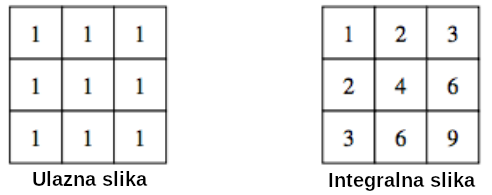
\includegraphics[width=8cm]{integral_image1}
  \caption{Primer integralne slike}
  \label{IntegralImage_img1}
\end{figure}

Piksele integralne slike je moguće računati u paraleli, ili
sekvencijalno. Izbor algoritma za računanje integralne slike značajno utiče na
performanse i potrebne hardverske resurse. \\
U paralelnoj implementaciji cena je
više pristupa memoriji i više potrebnih sabirača, dok je kod sekvencijalne
implementacije manja brzina. \\

Osobina koja integralnu sliku čini pogodnu za korišćenje u Viola-Jones algoritmu
je da je za računanje bilo koje pravougaone površine unutar integralne slike
potrebno 2 sabiranja i 2 oduzimanja.

\begin{figure}[h]
  \centering
  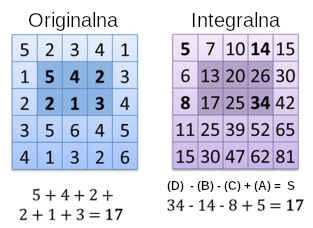
\includegraphics[width=8cm]{integral_image2}
  \caption{Primer računanja površine pravougaonika \cite{IntegralImage1_web}}
  \label{IntegralImage_img2}
\end{figure}

Na slici (\ref{IntegralImage_img2}) je prikazano računanje površine pravougaonika na
originalnoj slici i na integralnoj slici.
Kao što se može videti za površinu pravougaonika MxN na originalnoj slici nam je
potrebno MxN sabiranja. \\
Dok je kod integralne slike broj operacija 2 sabiranja i 2
oduzimanja i ne zavisi od dimenzija pravougaonika.

\begin{equation}
  \Scale[1.4]{\sum\limits_{(x,y)\in ABCD} i(x,y)=ii(D)+ii(A)-ii(B)-ii(C)}
  \cite{Cen2016StudyOV}
  \label{IntegralImage_eq2}
\end{equation}
\newpage

\section{OpenCV modeli} \label{opencv_model}

OpenCV je biblioteka koja sadrži implementacije velikog broja algoritama za
obradu slike.
OpenCV sadrži alat za AdaBoost treniranje kaskadnog klasifikatora kao i implementaciju
detektora objekata pomoću Viola-Jones algoritma. \\
Pored toga OpenCV sadrži istrenirane i testirane modele klasifikatora\footnote{\url{https://github.com/opencv/opencv/tree/master/data/haarcascades}}.
\cite{OpenCV_docs} \\

\noindent
OpenCV istrenirane modele skladišti u .xml fajlove koji sadrže sledeće
informacije o modelu:

\begin{itemize}
	\item Dimenzija obeležja (\emph{height, width})
	\item Broj etapa (\emph{stageNum})
	\item Maksimalan broj obeležja u etapi (\emph{maxWeakCount})
	\item Informacije o etapama (\emph{stages})
    \begin{itemize}
    \item Broj obeležja u etapi (\emph{maxWeakCount})
    \item Prag etape (\emph{stageThreshold})
    \item Informacije o obeležjima (\emph{weakClassifiers})
      \begin{itemize}
      \item Prag obeležja (\emph{internalNodes})
      \item Vrednosti listova (\emph{leafValues})
      \end{itemize}
    \end{itemize}
	\item Informacije o obeležjima (\emph{features})
    \begin{itemize}
    \item Koordinate i težine tačaka pravougaonika (\emph{rects}). \\
      Svako obeležje može imati 2 ili 3 pravougaonika. \\
      Prve 2 vrednosti liste rects su x i y koordinate gornje leve tačke, \\
      treća i četvrta vrednost širina i visina pravougaonika,  \\
      poslednja vrednost je težina pravougaonika.
    \end{itemize}
\end{itemize}

\subsection{OpenCV model za frontalna lica} \label{haarcascade_frontal_sec}

Često korišćeni model za detekciju lica je
\texttt{\detokenize{haarcascade_frontalface_default.xml}}\footnote{\url{https://github.com/opencv/opencv/blob/master/data/haarcascades/haarcascade_frontalface_default.xml}}. \\
Ovaj model se koristi za frontalnu detekciju lica. \\
Neke njegove karakteristike su:
\begin{itemize}
\item Dimenzija obeležja: 24x24
\item Broj etapa: 25
\item Maksimalan broj obeležja u etapi: 211
\item Ukupan broj obeležja: 2913
\end{itemize}

\noindent
Rezultati detekcije ovog modela mogu se videti na
slikama(\ref{sixfaces_scaled},\ref{overexposed_light},\ref{underexposed_light},\ref{rotation_variance},\ref{rotated_res})
iz sekcije \ref{viola_jones_introduction}.
\newpage

\part{Hardverska implementacija}
\section{Sažetak}

Ovaj projekat sadrži:
\begin{itemize}
  \item Projektovanje arhitekture hardverskog akceleratora za Viola-Jones algoritam opisam u delu \ref{viola_jones_algorithm}.
  \item Pisanje specifikacije u Python i C programskom jeziku za izvršavanje i
    pomoć pri particionisanju i projektovanju hardvera.
  \item Pisanje HDL modela za sintezu u SystemVerilog RTL metodologiji i
    \PyGears{} metodologiji.
  \item Pisanje verifikacionog okruženja u SystemVerilog \UVM{} i Python PyGears
    okruženju.
  \item Poređenje dve metodologije i analiza prednosti i mane obe metodologije.
  \item Poređenje komercijalnog \QuestaSim{} simulatora i besplatnog open-source
    \Verilator{} simulatora.
  \item Implementacija projektovanog IP jezgra na \ZTurn{} sa Zynq
    7020 SoC.
  \item Pisanje Linux Kernel drajvera i korisničke aplikacije za korišćenje
    jezgra za detekciju lica na Xilinx Zynq platformi.

\end{itemize}
\newpage
\section{Specifikacije za izršavanje}

Prilikom projektovanja hardverske arhitekture određenog algoritma preporučljivo
je prvo implementirati algoritam u softveru kako bi se algoritam bolje shvatio. \\
Postoje metodologije koje definišu potrebne korake prilikom projektovanja
digitalnih sistema, jedna takva metodologija je \gls{esl}.
U ovom radu nije korišćena ova metodologija već je softverska
specifikacija napisana u C++ i Python jeziku. \\
Iz ovih specifikacija dobijeno je bolje razumevanje algoritma i naznake o
mogućnosti paralelizna određenih delova algoritma i particionisanja komponenti
sistema. \\

\begin{figure}[H]
  \centering
  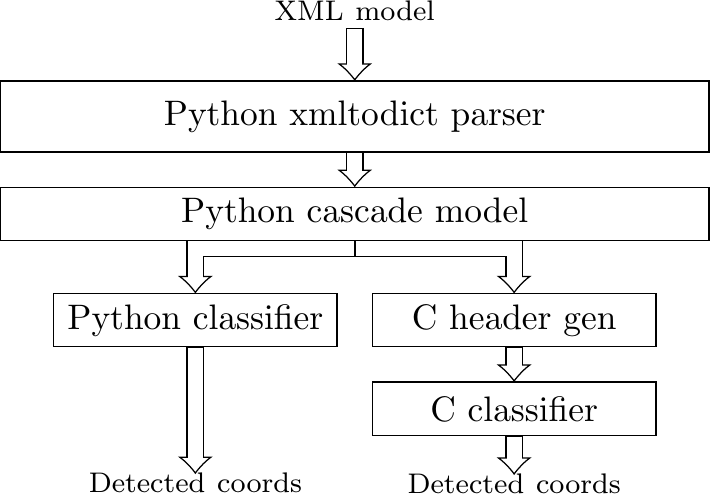
\includegraphics[width=0.9\linewidth]{bdp/sw_arch/sw_arch1.png}
  \caption{Veza Python modela sa XML modelom i C specifikacijom}
  \label{sw_arch_spec1}
\end{figure}

Na slici(\ref{sw_arch_spec1}) prikazana je struktura modela u slučaju Python i C
klasifikatora. \\

\noindent
Na ulazu se nalazi \gls{xml} model dobijen treniranjem pomoću OpenCV biblioteke opisan u sekciji
\ref{opencv_model}. \\
Parsiranje XML modela se rešava u Python-u.
Zbog velikog broja Python paketa dostupnih sa gotovim rešenjima za većinu softverskih problema, problem
parsiranja XML fajla se može rešiti korišćenjem paketa xmltodict\footnote{\url{https://pypi.org/project/xmltodict/}}. \\
\emph{Xmltodict} parsira XML fajl i skladišti ga u Python dictionary. \\
Implementirane su klase \emph{CascadeClass}, \emph{StageClass}, \emph{FeatureClass} i
\emph{RectClass}
\footnote{\texttt{\detokenize{cascade_classifier/python_model/cascade.py}}} koje
predstavljaju abstraktni Python model modela kaskadnog klasifikatora. \\

Napisana je i Python implementacija Viola-Jones algoritma koja koristi Python
model klasifikatora i koristi se kao specifikacija za izvršavanje. \\

Python model klasifikatora može da generiše \emph{C++} reprezentaciju modela
klasifikatora i sačuva ih u Header fajlove. \\
Ovim je izbegnuto parsiranje XML fajlova C++ jezikom, pošto je ovaj zadatak
mnogo jednostavnije odraditi u Python-u. \\
C++ implementacija Viola-Jones algoritma koristi ovako generisan model
klasifikatora.
\newpage
\pgfdeclarelayer{background}
\pgfdeclarelayer{foreground}
\pgfsetlayers{background,main,foreground}

\tikzstyle{cloud1} = [draw=black, thick, fill=red!20, minimum hegiht = 1em]
\tikzstyle{block_l} =[draw, text centered, fill=blue!15, minimum width=3cm, minimum height=3.5cm]
\tikzstyle{block_m} =[draw, text centered, fill=blue!15, minimum width=2.5cm, minimum height=2cm]
\tikzstyle{block_s} =[draw, text centered, fill=blue!15, minimum width=2cm, minimum height=1.5cm]
\tikzstyle{line} = [draw, decoration={markings,mark=at position 1 with {\arrow[scale=2.2,black]{>}}},
    postaction={decorate},
    shorten >=0.4pt]

\begin{tikzpicture}[thick]
  \node [block_l] (img_ram) {IMG RAM};
  \node [coordinate, above = 0cm of img_ram, yshift=-0.5cm, xshift=1.5cm] (img_ram_addr_in){};
  \node [coordinate, left =2.0cm of img_ram] (img_in){};
  \node [coordinate, left = 0cm of img_ram] (img_ram_img_in){};
  \node [coordinate, right = 0cm of img_ram] (img_ram_img_out){};

  \node [block_m, above right = +1cm and 0.2cm of img_ram] (rd_addrgen) {rd\_addrgen};
  \node [coordinate, below = 0cm of rd_addrgen] (rd_addr_addr_out){};

  \node [block_m, above right = -1.75cm and 2.5cm of img_ram ] (ii_gen) {ii\_gen};
  \node [coordinate, left = 0cm of ii_gen] (ii_gen_in){};
  \node [coordinate, right = 0cm of ii_gen] (ii_gen_out){};
  \node [block_m, below = 0.25cm of ii_gen ] (sii_gen) {sii\_gen};
  \node [coordinate, left = 0cm of sii_gen] (sii_gen_in){};
  \node [coordinate, right = 0cm of sii_gen] (sii_gen_out){};

  \node [block_s, right = 1.25cm of sii_gen ] (stddev) {stddev};
  \node [coordinate, above left = -0.25cm and 0cm of stddev] (stddev_ii){};
  \node [coordinate, above left = -0.75cm and 0cm of stddev] (stddev_sii){};
  \node [coordinate, right = 0cm of stddev] (stddev_out){};

  \node [block_m, right = 1.0cm of ii_gen ] (frame_buffer) {frame\_buffer};
  \node [coordinate, left = 0cm of frame_buffer] (frame_buffer_in){};
  \node [coordinate, above left = -0.5cm and 0cm of frame_buffer] (frame_buffer_rect_addr){};
  \node [coordinate, right = 0cm of frame_buffer] (frame_buffer_out){};

  \node [block_m, above = 1.0cm of frame_buffer ] (features_mem) {features\_mem};
  \node [coordinate, left = 0cm of features_mem] (rects_addr){};
  \node [coordinate, right = 0cm of features_mem] (rects_weights){};

  \node [block_l, fill=red!15, above right = -3.5cm and 1cm of frame_buffer] (classifier) {\huge Classifier};
  \node [coordinate, above left = -1cm and 0cm of classifier] (classifier_ii){};
  \node [coordinate, above left = -2.5cm and 0cm of classifier] (classifier_stddev){};
  \node [coordinate, above left = -0.5cm and 0cm of classifier] (classifier_weights){};
  \node [coordinate, above right = -1.0cm and 0cm of classifier] (detected_addr){};
  \node [coordinate, above right = -2.5cm and 0cm of classifier] (irq){};

  %% group %%
 \begin{pgfonlayer}{background}
  \node[inner sep=7pt, fill=yellow!25, rounded corners, inner ysep =30pt, draw, thick,fit=(img_ram) (rd_addrgen) (ii_gen) (features_mem) (sii_gen) (frame_buffer) (stddev) (classifier)] (ip_core) {};
  \node[above left] at (ip_core.south east) {\huge Cascade Classifier IP core};
\end{pgfonlayer}

  % arrows
  \path [line] (rd_addr_addr_out)  |- (img_ram_addr_in) node[transition, xshift=0.8cm, yshift=0.25cm] {rd\_addr};
  \path [line] (img_in) node[transition, yshift=0.25cm, xshift=0.65cm]{\large img\_in} -- (img_ram_img_in);
  \path [line] (img_ram_img_out) node[transition, yshift=0.2cm, xshift=0.9cm] {img\_out} -- +(1.75cm, 0cm) |- (ii_gen_in);
  \path [line] (img_ram_img_out) -- +(1.75cm, 0cm) |- (sii_gen_in);
  \path [line] (ii_gen_out) -- +(0.5cm, 0cm) node[transition, yshift=0.2cm, xshift=0cm] {ii} |- (stddev_ii);
  \path [line] (sii_gen_out) -- +(0.5cm, 0cm)  node[transition, yshift=0.2cm, xshift=0cm] {sii} |- (stddev_sii);
  \path [line] (ii_gen_out) |- (frame_buffer);
  \path [line] (frame_buffer_out) node[transition, yshift=+0.2cm, xshift=0.5cm] {fb\_ii} |- (classifier_ii);
  \path [line] (stddev_out) -- +(0.5cm, 0) node[transition, yshift=-0.2cm, xshift=0.1cm] {stddev} |- (classifier_stddev);
  \path [line] (rects_addr) node[transition, yshift=+0.2cm, xshift=-1.1cm] {rects\_addr}  -- +(-0.5cm, 0cm) |- (frame_buffer_rect_addr);
  \path [line] (rects_weights) node[transition, yshift=+0.2cm, xshift=+1.2cm] {rects\_weights}  -- +(+0.5cm, 0cm) |- (classifier_weights);
  \path [line] (detected_addr) -- +(3.0cm, 0cm) node[transition, yshift=0.25cm, xshift=-1.1cm]{\large detect\_addr} ;
  \path [line] (irq) -- +(3.0cm, 0cm) node[transition, yshift=0.25cm, xshift=-0.4cm]{\large irq} ;
\end{tikzpicture}

\newpage
\newpage

\bibliography{bibliography}
\bibliographystyle{IEEEtran}

\end{document}